\section{Using ML for the Keyspace}
\label{sec:ml-for-the-keyspace}

We prove in the previous section that an efficient policy, based on the read
burstiness at the beginning of the run,  exists for \(\Delta_1\) on 8 nodes,
but we cannot re-do this analysis for every workload, system, and parameter
permutation.  Fortunately, Section~\S\ref{sec:parsplice-keyspace-analysis}
shows that the keyspace size and activity is structured. Rather than finding
policies by hand again for every cluster size, growth rate, and temperature, in
this section we use machine learning (ML) to inform the Mantle policy engine.

In general, ML excels at both pruning large design spaces and classification.
Our keyspace analysis in Section~\ref{sec:parsplice-keyspace-analysis}
demonstrates a large design space and Figure~\ref{fig:motivation-regimes} shows
4 workload regimes: one plateau of redundant reads at the beginning, decreasing
requests per second, and then two plateaus of steady requests per second. We
start with a simple clustering algorithm to attack this multi-dimensional
design space problem and detect workload regimes.

% implementation: 
We feed the read request rate from the \(\Delta_1\) and \(\Delta_2\) runs in
Figure~\ref{fig:motivation-regimes} into the K-means clustering algorithm as
(timestamp, ops/second) tuples\footnote{Note that the magnitudes are different
because Figure~\ref{fig:motivation-regimes} was run with keyspace tracing on
and across less nodes which reduces performance}. We weight the timestamp and
ops/second equally and set the number of clusters to be 4.  We chose this
initial K  based on visual inspection of Figure~\ref{fig:motivation-regimes}.
Knowing that the setup parameters transform the request rates temporally or
spatially, this same initial K should work for all setups. Once the algorithm
identifies the workload regimes, we select the start of the third regime as the
point to switch to a fixed sized cache because the request rate has lowered to
sustainable levels for the persistent database.

We plot throughput over time in Figure~\ref{fig:futurework-regimes} and
color each point with its assigned group. The black stars are the centroids,
also known as the center of K-means groups.  We run the algorithm for a variety
of request rate traces but only show the setups from
Figure~\ref{fig:motivation-regimes}. We also annotate the graphs with the
suggested cache size, which is calculated by looking up the timestamp for the
third regime that corresponds to the keyspace size in our performance counters.

% results: 1. identifies 4 phases, 2. picks different timestamps for the third
% regime, suggests proper key values.
The algorithm properly identifies the 4 workload phases: the plateau of
redundant reads, the phase with a large decrease in request rate, and the two
plateaus of steady read requests. Our implementation also selects different
timestamps for the start of the third regime, which aligns with our keyspace
analysis and our assertion that the growth parameters affect how long it takes
the workload to reach a certain phase.  Finally, the algorithm chooses
reasonable values for the key cache size. The \(\Delta_1\) growth rate selects
a 55K key cache size, which is between the threshold we chose using brute force
for the high watermark (100K) and lower cache size (10K) in our dynamic policy.
Note that this result does not validate our claims about ML, rather it is a
promising development and suggests that we may avoid lengthy parameters sweeps
for ParSplice in the future.

\begin{figure}[t]
\noindent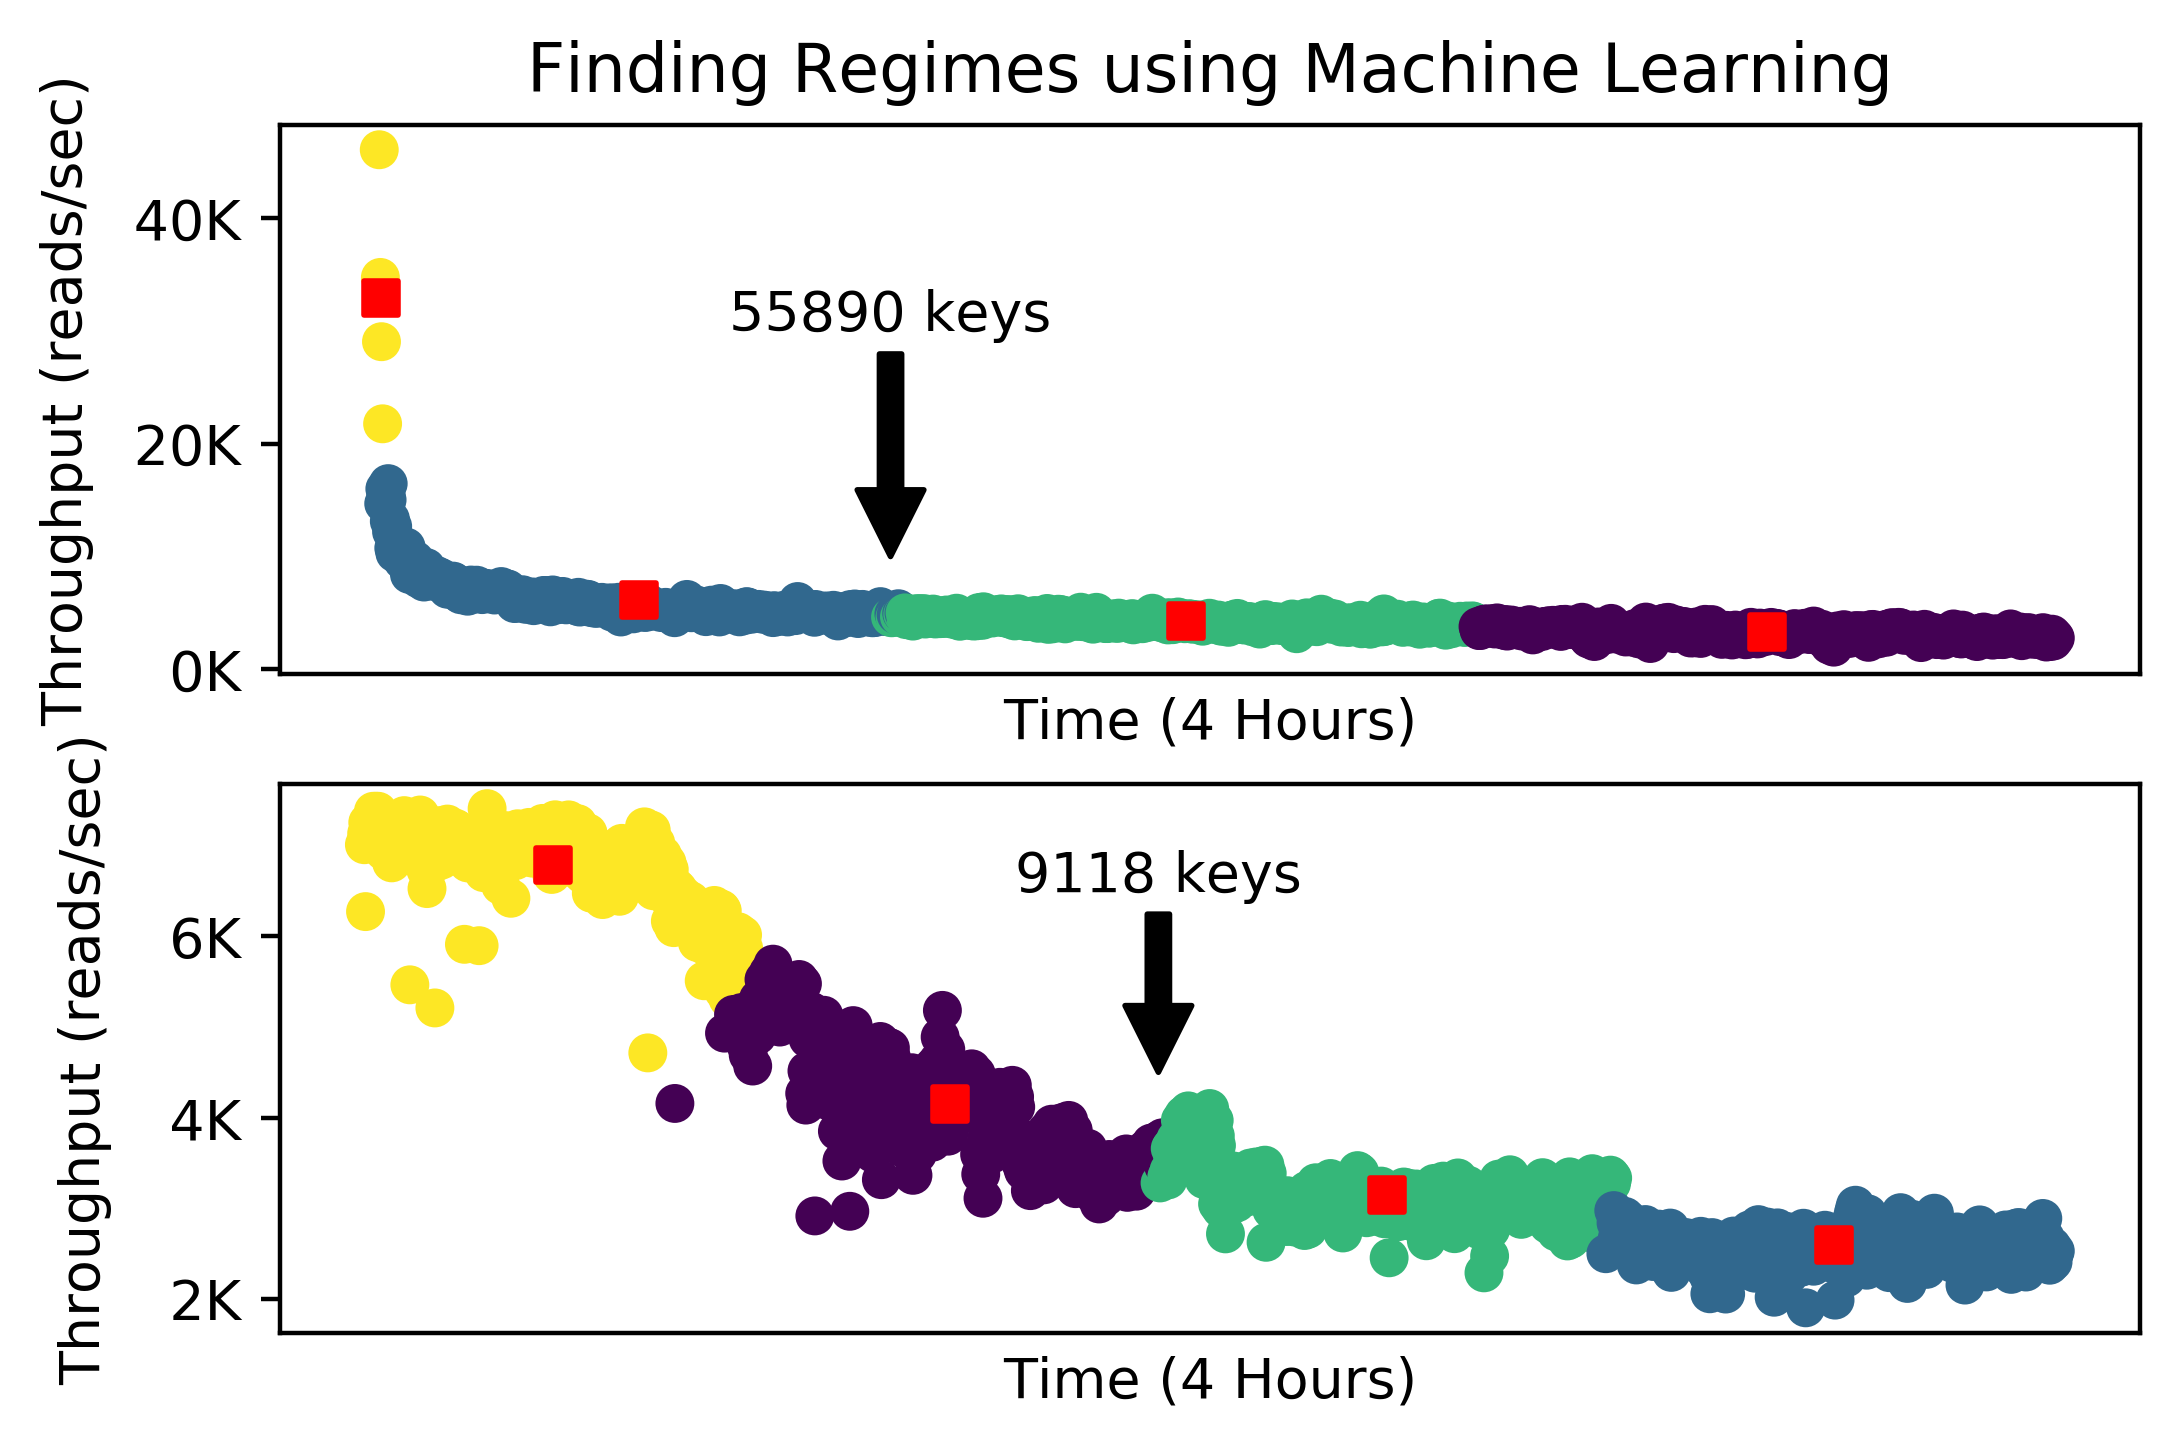
\includegraphics[width=0.5\textwidth]{figures/futurework-regimes.png}\\
  \caption{Learning the workload regimes with K-means clustering helps pick
  cache size thresholds that can be fed into a dynamic load balancing policy
  engine, like Mantle. Specifying 4 clusters and selecting the third for
  informing the policy switch returns keyspace size thresholds similar to the
  values we found by hand in
  Section~\S\ref{sec:the-need-for-dynamic-load-balancing-policies}.
\label{fig:futurework-regimes}}
\end{figure}
